\documentclass{article}

\usepackage[T1]{fontenc}
\usepackage{siunitx}
\usepackage[polish]{babel}
\usepackage[utf8]{inputenc}
\usepackage{float}
\usepackage{graphicx}
\usepackage{amsmath}
\usepackage{siunitx}
\usepackage{longtable}
\oddsidemargin 0pt
\evensidemargin 0pt
\marginparwidth 40pt
\marginparsep 10pt
\topmargin -20pt
\headsep 10pt
\textheight 8.7in
\textwidth 6.65in
\linespread{1.2}

\title{Sprawozdanie z Laboratorium 8.}
\author{Piotr Lewandowski \and Dymitr Lubczyk \and Krzysztof Tabeau }
\date{\today}
\begin{document}
\maketitle
\begin{tabular}{|l|l|}
\hline
Autorzy             & Dymitr Lubczyk                    \\
                    & Krzysztof Tabeau                  \\
                    & Piotr Lewandowski                 \\
Wydział             & Matematyki i Nauk Informacyjnych  \\
Numer Zespołu       & 19                                \\
Data laboratorium   & 17:15 29.06.2020                  \\
Numer laboratorium  & 8                                 \\
Prowadzący          & dr inż. Izabela Duncin         \\
\hline
\end{tabular}

\section{Materiały i metody}
Wahadło matematyczne skonstruowaliśmy w następujący sposób:
\begin{itemize}
    \item Metalowy pręt z dziurką i wyżłobieniem położyliśmy na pawlaczu, tak aby częściowo wystawał.
    \item Na ukrytą część pręta położyliśmy ciężki przedmiot (walizkę), aby mieć pewność że nie będzie żadnych niepożądanych przemieszczeń
    \item Przez dziurkę w pręcie przełożyliśmy nić, którą przywiązaliśmy do długopisu
    \item Długopis położyliśmy w wyżłobieniu, tak aby jego ruch był zablokowany
    \item Do drugiego końca nici przywiązaliśmy pionek z gry planszowej, którego kształt jest zbliżony do kuli
    \item Przykleiliśmy kątomierz do pręta do ułatwienia pomiarów
\end{itemize}
Do pomiarów używaliśmy następujących narzędzi:
\begin{itemize}
    \item Kątomierz - przedziałka co jeden stopień. Niepewność eksperymentatora to dwa stopnie, ponieważ kamera nagrywająca eksperyment była lekko przesunięta względem środka kątomierza.
    \item Metrówka - przedziałka co 1mm. Niepewność eksperymentatora względem długości wahadła to 5mm, ponieważ eksperyment był w warunkach domowych i nie zawsze można było łatwo skrócić nić do zamierzanej długości oraz metrówka nie była w najlepszym stanie.
    \item Linijka - przedziałka co 1mm. Niepewność eksperymentatora względem ciężarka to 0mm. Pomiary były przeprowadzane w statycznych i pewnych warunkach.
    \item Kamera - oprócz ułatwienia pomiarów, kamera również służyła do mierzenia czasu.Dokładność pomiaru czasu jest co do 1ms, ale niepewność eksperymentatora jest wielkości 211ms. Zmierzyliśmy ją wciskając start i pauzę od razu po sobie.
\end{itemize}
\clearpage
\begin{figure}[H]
\centerline{\includegraphics[scale=0.07]{stacja.jpg}}
\caption{Domowe wahadło matematyczne}
\end{figure}
\begin{figure}[H]
\centerline{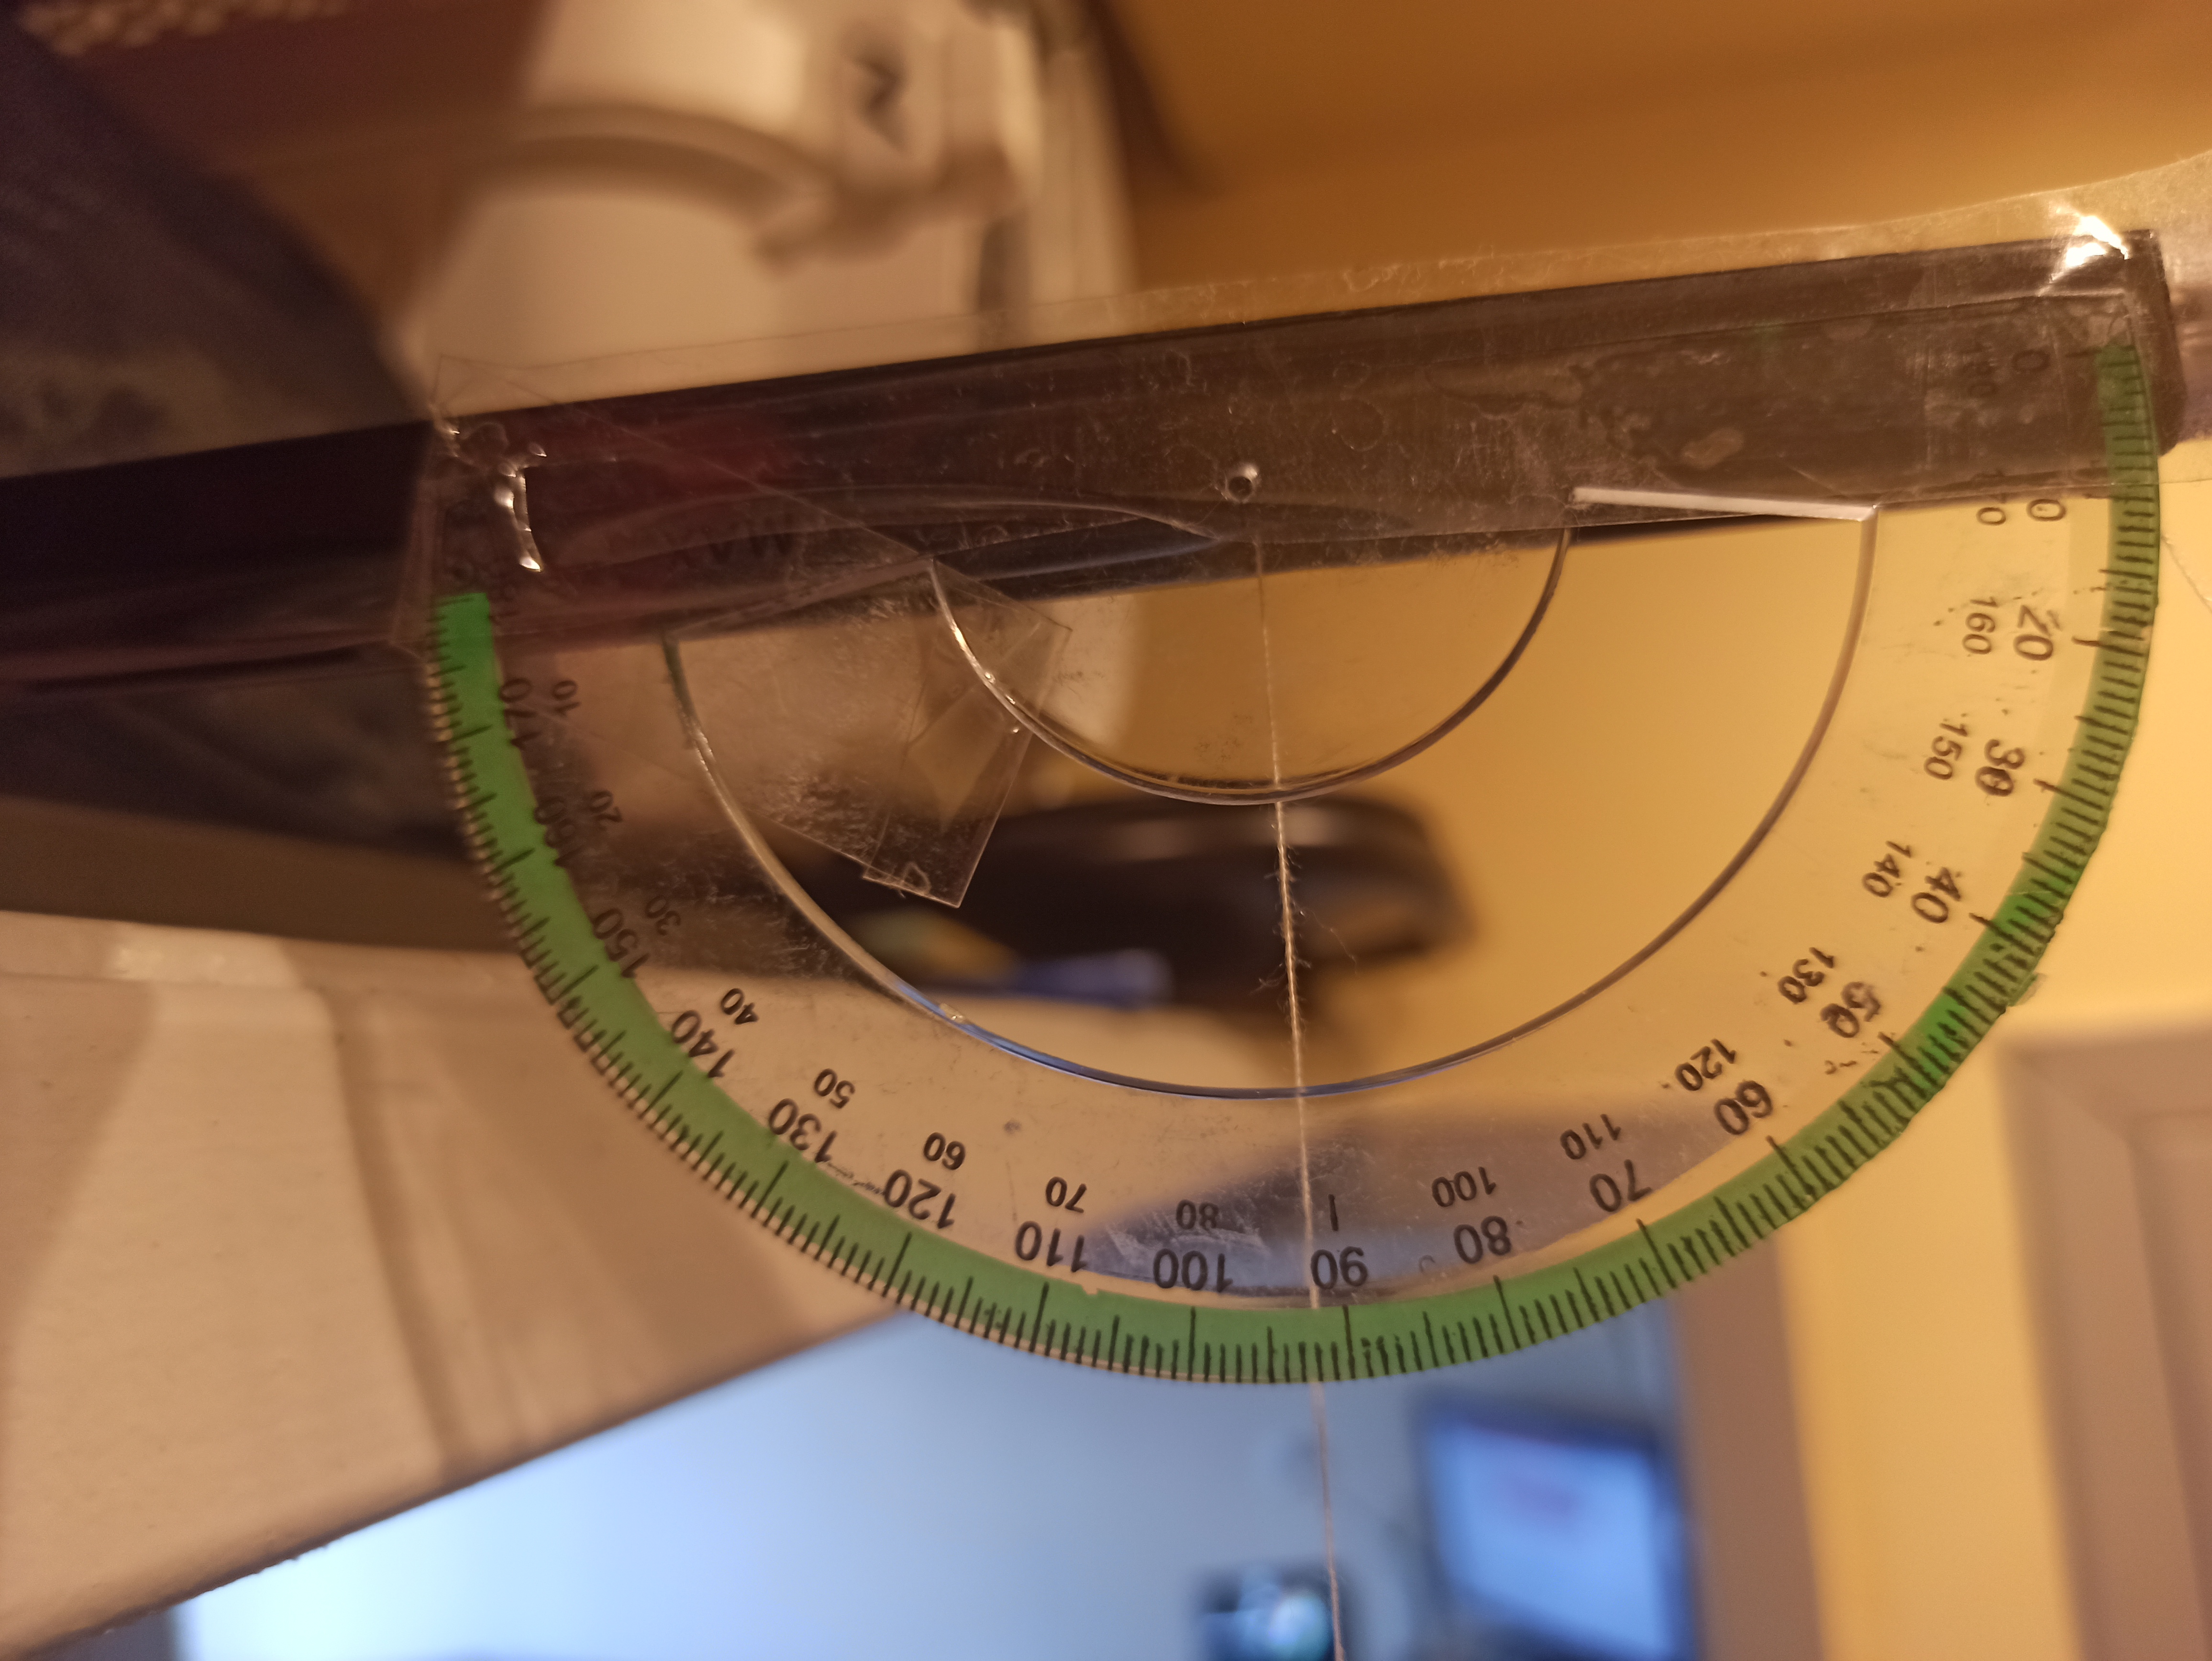
\includegraphics[scale=0.07]{katomierz.jpg}}
\caption{Kątomierz}
\end{figure}
\begin{figure}[H]
\centerline{\includegraphics[scale=0.07]{linijka.jpg}}
\caption{Metrówka}
\end{figure}
\begin{figure}[H]
\centerline{\includegraphics[scale=0.07]{lini.jpg}}
\caption{Linijka}
\end{figure}
\clearpage

\noindent Doświadczenie przeprowadzaliśmy w dwie osoby. Jedna osoba wychylała wahadło za pomocą książki, tak aby było równo i aby wahadło poruszało się w jednej osi, a druga osoba instruowała pierwszą jak bardzo ma je wychylić, ponieważ tylko ta druga osoba widziała odchylenie na kątomierzu. 
Następnie pierwsza osoba puszczała wahadło i kamera nagrywała ruch i czas ruchu wahadła.
W przypadku skracania nici przy pomiarach zależności okresu wahadła od jego długości. Jedna osoba nawijała nić na długopis, a druga naciągała metrówkę i sprawdzała czy jest już odpowiednia długość. 

\clearpage
\section{Wprowadzenie teoretyczne}
Przeprowadzane doświadczenie składa się z dwóch części:
\begin{itemize}
    \item Badanie zależności okresu drgań wahadła matematycznego od kąta
wychylenia
    \item Badanie zależności okresu drgań wahadła różnicowego od
zmiany długości nici
\end{itemize}

\subsection{Wahadło matematyczne}
Teoretycznym modelem, z którego pomocą można opisać ruch skonstruowanego przez nas wahadła jest tak zwane wahadło matematyczne, czyli punkt materialny zawieszony na nieważkiej i nierozciągliwej nici, poruszający się po okręgu. W tym modelu brana jest pod uwagę jedynie siła grawitacji oraz siła reakcji nici. Celem tej części doświadczenia jest zaobserwowanie anharmoniczności wahadła matematycznego, czyli zależności okresu drgań wahadła od kąta maksymalnego wychylenia, która w poniższym wzorze na okres drgań jest reprezentowana przez czynnik $f(\alpha)$.
\begin{gather*}
    T = 2 \pi \sqrt{\frac{l}{g}} f(\alpha) \\
    S = l \alpha \\
    m \frac{d^2S}{dt^2} = -m g * sin \alpha \\
    \frac{d^2 \alpha}{dt^2} = - \frac{g}{l} sin \alpha
\end{gather*}

\subsection{Wahadło różnicowe}
W tym ćwiczeniu konieczna jest możliwość zmiany długości wahadła, więc model wahadła matematycznego możemy o tę opcję rozszerzyć, tworząc wahadło różnicowe. Wpływ tej zmiany na okres ruchu wahadła przedstawiają poniższe wzory.
\begin{gather*}
    \delta l = l_0 - l_i \\
    \delta T = T_0^2 - T_i^2 \\
    T_i = 2 \pi \sqrt{\frac{l_i}{g}} f(\alpha) \\
    T_0^2 - T_i^2 = \frac{4\pi^2}{g}f^2(\alpha) (l_0-l_i)
\end{gather*}

W celu wyznaczenia przyspieszenia grawitacyjnego wykorzystamy ostatnią z powyższych zależności w następujący sposób:
\begin{gather*}
    y = ax \\
    y = \delta T \\
    g = a = \frac{4\pi^2}{g}f^2(\alpha) \\
    x = \delta l 
\end{gather*}

\clearpage
\section{Wyniki}
\subsection{Pomiary}
Do badania zależności okresu drgań wahadła od kąta wychylenia użyliśmy wahadła o długości 1m ( z niepewnością 2,958 mm) i otrzymaliśmy następujące dane: 
\begin{table}[h!]
    \centering
    \begin{tabular}{|c|c|c|c|c|} \hline
    $\alpha_{p}$ & $\alpha_{k}$ & $\overline{\alpha}$ & 5T [s] & $\overline{T} [s]$ \\ \hline
    10	&	6	&	8	&	9,47	&	1,894	\\
    12	&	7	&	9,5	&	9,72	&	1,944	\\
    14	&	7	&	10,5	&	9,711	&	1,9422	\\
    16	&	8	&	12	&	9,945	&	1,989	\\
    18	&	8	&	13	&	10,771	&	2,1542	\\
    20	&	9	&	14,5	&	10,035	&	2,007	\\
    22	&	9	&	15,5	&	10,257	&	2,0514	\\
    24	&	10	&	17	&	10,846	&	2,1692	\\
    26	&	10	&	18	&	10,317	&	2,0634	\\
    28	&	10	&	19	&	9,553	&	1,9106	\\
    30	&	11	&	20,5	&	10,118	&	2,0236	\\ \hline
    \end{tabular}
\end{table}\\
Z następującymi niepewnościami:
\begin{table}[h!]
    \centering
    \begin{tabular}{|c|c|c|c|c|} \hline
    $\alpha_{p}$ & $\alpha_{k}$ & $\overline{\alpha}$ & 5T & $\overline{T}$ \\ \hline
    1,290	&	1,290	&	0,91287	&	122,398ms	&	24,480ms	\\ \hline
    \end{tabular}
\end{table}
Dane zaprezentowane na wykresie:
\begin{figure}[H]
\centerline{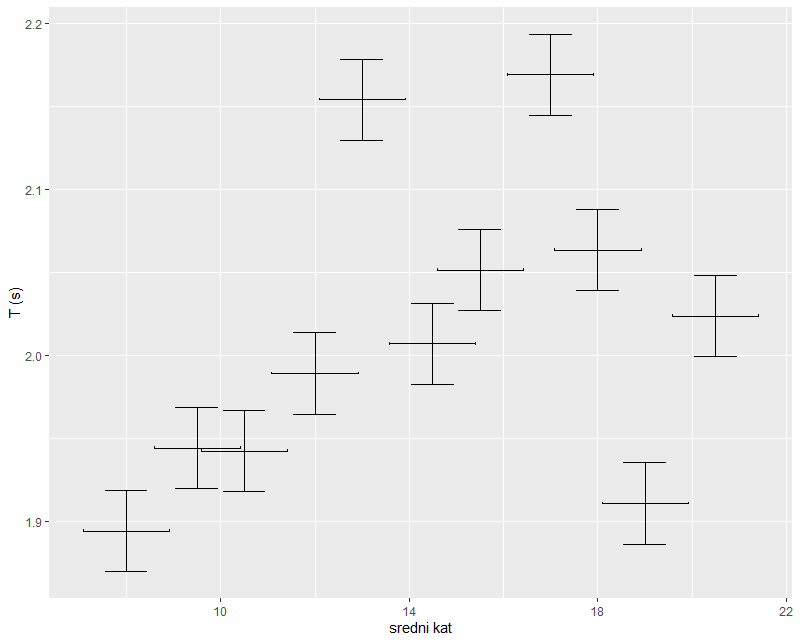
\includegraphics[scale=0.7]{lab81.png}}
\end{figure}
Do badania zależności okresu drgań wahadła od zmiany długości zebraliśmy poniższe dane:
\begin{table}[h!]
    \centering
    \begin{tabular}{|c|c|c|c|} \hline
    $\Delta l$ [cm] & $ 5T [s]$  & $\overline{T}$ [s] & $\Delta T = T^2_{0} - T^2_{i}$ \\ \hline
    0	&	10,035	&	2,007	&	0	\\
    4	&	9,656	&	1,9312	&	0,29851556	\\
    8	&	9,503	&	1,9006	&	0,41576864	\\
    12	&	9,437	&	1,8874	&	0,46577024	\\
    16	&	9,124	&	1,8248	&	0,69815396	\\
    20	&	8,767	&	1,7534	&	0,95363744	\\
    24	&	8,528	&	1,7056	&	1,11897764	\\
    28	&	8,446	&	1,6892	&	1,17465236	\\
    32	&	8,266	&	1,6532	&	1,29497876	\\
    36	&	8,017	&	1,6034	&	1,45715744	\\
    40	&	7,758	&	1,5516	&	1,62058644	\\ \hline
    \end{tabular}
\end{table}\\
Z następującymi niepewnościami:
\begin{table}[h!]
    \centering
    \begin{tabular}{|c|c|c|c|} \hline
    $\Delta l$ & $ 5T $  & $\overline{T}$ & Niepewność $\Delta T$\\ \hline
    4,1833 mm	&   122,398ms	&	24,480ms & 34,6195 ms	\\ \hline
    \end{tabular}
\end{table}
Dane zaprezentowane na wykresie:
\begin{figure}[H]
\centerline{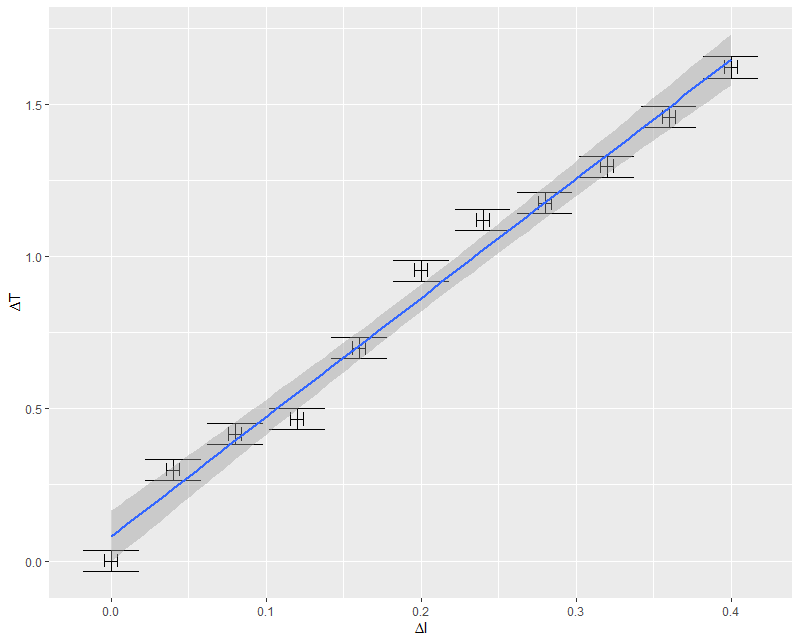
\includegraphics[scale=0.7]{lab82.png}}
\end{figure}
Powyższy liniowy wykres można opisać parametrami \textit{$a = 3.91221$} z odchyleniem standardowym równym \textit{0.15707} i \textit{$b = 0.08103$}.
Jak wiemy z teorii \textit{b} powinno być równe 0, a \textit{a} jest równe $\frac{4\pi^2}{g}* f(\alpha)$.
Wiedząc, że $\alpha = 20$ i $f(\alpha) = 1.008$, możemy wyliczyć, że $g = 10,249(411) \frac{m}{s^2}$ 

\clearpage
\section{Analiza i rachunek niepewności}
Niepewność liczyliśmy w następującymi wzorami:
\begin{gather*}
    u_{B}(\alpha_{P}) = u_{B}(\alpha_{K}) = u_{B}(\alpha) = \sqrt{\frac{\Delta \alpha^2 + \Delta \alpha_{e}^2}{3}} = \sqrt{\frac{1 + 5}{3}} = 1,290 \\
    u_{B}(5T) = \frac{\Delta T}{\sqrt{3}} + \frac{\Delta T_{e}}{\sqrt{3}} = \frac{1}{\sqrt{3}} + \frac{211}{\sqrt{3}} = 0,122398 s \\
    \overline{\alpha} = \frac{\alpha_{P} + \alpha_{K}}{2} \\
    u_{B}(\overline{\alpha}) = \sqrt{(\frac{\delta \overline{\alpha}}{\delta \alpha_{P}})^2 * u_{B}(\alpha)^2 + (\frac{\delta \overline{\alpha}}{\delta \alpha_{K}})^2 * u_{B}(\alpha)^2} 
    = u_{B}(\alpha) * \sqrt{\frac{1}{4} + \frac{1}{4}} = 0,91287 \\
    \overline{T} = \frac{5T}{5} \\
    u_{B}(\overline{T}) = \sqrt{(\frac{\delta \overline{T}}{\delta 5T})^2 * u_{B}(5T)^2} = \frac{1}{5} * u_{B}(5T) = 24,480 ms \\
    l = L + \frac{1}{2} d \\
    u_{B}(\overline{L}) = \sqrt{\frac{\Delta L^2 + \Delta L_{e}^2}{3}} = \sqrt{\frac{26}{3}} = 2,9439 mm \\
    u_{B}(\overline{d}) = \sqrt{\frac{\Delta d^2 + \Delta d_{e}^2}{3}} = \sqrt{\frac{1}{3}} = 0,5774 mm \\
    u_{B}(l) = \sqrt{(\frac{\delta l}{\delta L})^2 * u_{B}(L)^2 + (\frac{\delta l}{\delta d})^2 * u_{B}(d)^2} = 2,9580 mm \\
    \delta l = l_{P} - l_{K} \\
    u_{B}(l_{P}) = u_{B}(l_{K}) = u_{B}(l) \\
    u_{B}(\Delta l) = \sqrt{(\frac{\delta \Delta l}{\delta l_{P}})^2 * u_{B}(l)^2 + (\frac{\delta \Delta l}{\delta l_{K}})^2 * u_{B}(l)^2} = \sqrt{2} * u_{B}(l) = 4,1833 mm \\
    u_{B}(\Delta T) = \sqrt{(\frac{\delta \Delta T}{\delta T_{0}})^2 * u_{B}(T)^2 + (\frac{\delta \Delta T}{\delta T_{i}})^2 * u_{B}(T)^2} = \sqrt{2} * u_{B}(T) = 34,6195 ms \\
    u_a(g) = \sqrt{(\frac{\delta g}{\delta a})^2 * u(a)^2} = \frac{4\pi^2}{a^2} * f(\alpha)^2 * u(a) = 0,411 \frac{m}{s^2}\\
\end{gather*}
Doświadczenie było przeprowadzane w warunkach domowych bez przyrządów wysokiej jakości do mierzenia danych. Wahadło było wprowadzane w ruch przez człowieka, więc zawsze jest szansa na niedokładność, której się nie da zmierzyć. Przykładowo jeśli niechcący wprawi się wahadło w ruch lekko eliptyczny to wychylenie będzie obarczone błędem. Same przyrządy były obarczone dużą niepewnością co skutkuje w gorszych obliczaniach.

\clearpage
\section{Dyskusja wyników i wnioski}
W pierwszej części eksperymentu uzyskane przez nas wyniki dość znacznie odbiegają od wartości teoretycznych. Jest to spowodowane dużą niepewnością całego układu pomiarowego, wynikającej z jego prowizorycznej konstrukcji, błąd mógł się pojawić z powodów, których nie uwzględniliśmy w naszych obliczeniach, takich jak na przykład poruszanie się elementów urządzenia względem siebie, lub poruszanie się wahadła poza przewidzianą płaszczyzną. W drugiej części doświadczenia udało się nam uniknąć tego typu problemów i uzyskana przez nas charakterystyka jest zgodna z teoretycznymi przewidywaniami. Obliczona wartość przyspieszenia ziemskiego jest większa od rzeczywistej, jednak zważając na wykorzystaną metodę i narzędzia, jest to stosunkowo dobry wynik.
\end{document}

